\documentclass[sigconf]{acmart}
\renewcommand\footnotetextcopyrightpermission[1]{} % Removes the copyright block
\settopmatter{printacmref=false, printccs=false, printfolios=false} % Suppress ACM references
\pagestyle{plain} % Plain header and footer

% added
\usepackage{amsmath}
\usepackage{geometry}
\usepackage{array}
\usepackage{graphicx}  % For resizing the table

% Remove conference information
\acmConference{}{}{} % Clears conference name, location, and date
\acmYear{} % Clears year
\acmISBN{} % Clears ISBN
\acmDOI{} % Clears DOI

\begin{document}

\title{Equivariant Diffusion for Molecule Generation in 3D}

\author{Gaëtan Ecrepont}
\email{gaetan.ecrepont@polytechnique.edu}
\affiliation{%
  \institution{Ecole Polytechnique}
  \city{Paris}
  \country{France}
}

\author{Samson Gourevitch}
\email{samson.gourevitch@polytechnique.edu}
\affiliation{%
  \institution{Ecole Polytechnique}
  \city{Paris}
  \country{France}
}

\author{Samuel Sarfati}
\email{samuel.sarfati@ens-paris-saclay.fr}
\affiliation{%
  \institution{ENS Paris-Saclay}
  \city{Paris}
  \country{France}
}

\begin{abstract}
This paper discusses the work of Hoogeboom et. al \cite{edm} on 3D molecule generation using E(3) Equivariant Diffusion Models (EDM). We demonstrate the benefits of incorporating E(3)-equivariance in Graph Neural Networks (GNN) through a toy model experiment. Additionnally, we highlight the limitations of the paper and propose potential extensions.
\end{abstract}


\keywords{molecule generation, equivariant network, diffusion models, graph neural networks}


\begin{teaserfigure}
  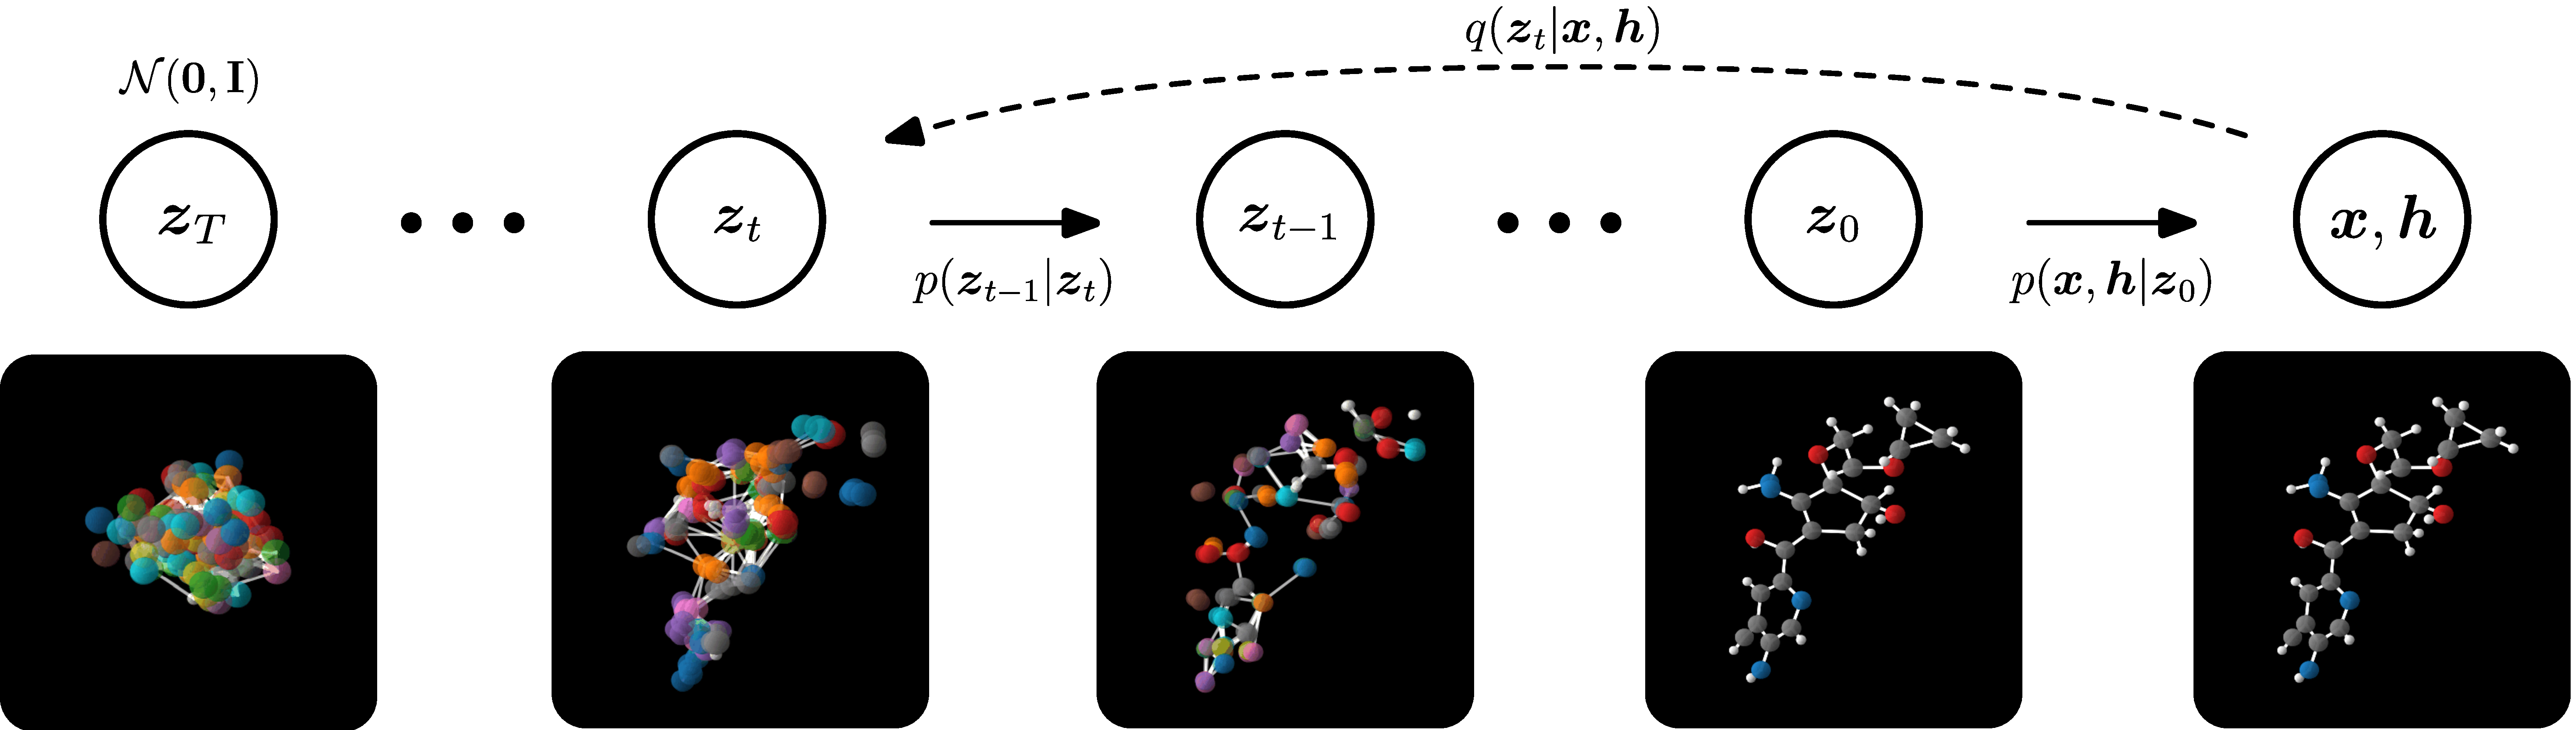
\includegraphics[width=\textwidth]{figures/overview_diffusion.pdf}
  \caption{Overview of the Equivariant Diffusion Model}
  \Description{Overview of the Equivariant Diffusion Model}
  \label{fig:teaser}
\end{teaserfigure}

\received{4 December 2024}

\maketitle

\section{Introduction} %% 1) Context

The paper is organized as follows: Section 1 contextualizes 3D molecule generation and presents Hoogeboom et. al's approach, Section 2 motivates and defines the E(3) Equivariant Diffusion Model (EDM), Section 3 discusses the limitations and potential extensions of the model and Section 4 presents the results of our experiments on a toy model.

\subsection{Molecule Generation in 3D}
Molecular design in three-dimensional space represents a pivotal challenge in computational biology and related fields. The primary objective involves generating molecular conformations that align with real-world chemical and physical properties, such as stability and functional relevance. However, achieving this objective is fraught with technical difficulties. These include accurately modeling interatomic forces, ensuring geometric coherence, and capturing complex interactions. Historically, advancements such as classical molecular dynamics and quantum chemical methods provided insights into molecular structures, but they were computationally intensive and limited in scalability.

The advent of machine learning has offered promising alternatives. Deep generative models can now synthesize molecular structures by learning implicit rules from large datasets, but many challenges remain unresolved. Existing models often fail to generalize to complex, larger molecules or exhibit instability in the generated conformations. Additionally, real-world applications demand molecules optimized for specific properties, such as drug discovery targets or material design requirements, necessitating models that combine precision with adaptability. Success in these domains can unlock transformative innovations, including the design of new drugs, advanced materials, and sustainable catalysts.

\subsection{Existing approaches}
Existing approaches to 3D molecular generation encompass a variety of methods. Notably, among these, autoregressive models and continuous-time normalizing flows have implemented E(n) equivariant layers, which leverage geometric symmetries to enhance the generation of 3D structures. Autoregressive models, such as those introduced by \cite{gebauer2018generating} and \cite{gebauer2019symmetry}, generate molecules atom by atom in a predefined order. While effective for smaller molecules, these models impose artificial constraints that complicate scalability and limit the flexibility of atomic arrangements. Furthermore, sampling efficiency decreases as molecule size increases, a challenge highlighted in \cite{xu2021anytime}.

Continuous-time normalizing flows, exemplified by methods like \cite{kohler2020equivariant} and E-NF \cite{garcia2021n}, offer an alternative by transforming simple distributions into molecular conformations through invertible transformations. These methods inherently handle 3D coordinates but at a significant computational cost due to their reliance on solving differential equations. This restricts their applicability to small molecules or datasets with limited diversity. Additionally, while these models leverage geometric invariances, their performance often remains constrained by their underlying architectures.

Other generative methods have also emerged, such as score-based models (e.g. \cite{shi2021learning}, \cite{xu}), which demonstrate strong performance in coordinate prediction by incorporating geometric symmetries but are often limited to specific conformer generation tasks. Grid-based approaches (e.g. \cite{ragoza2020learning}) use 3D convolutional networks to predict molecular structures mapped onto fixed grids but struggle with precise geometric fidelity. Hybrid models, like those by \cite{ganea2021geomol}, combine graph-based and coordinate-based generation for enhanced representation but increase model complexity.

These methods set important benchmarks but lack robustness in scaling to larger molecules, addressing real-world dataset diversity, or balancing computational efficiency and expressiveness. The limitations of these approaches emphasize the need for novel methodologies capable of direct 3D generation while ensuring scalability, stability, and efficiency.

\subsection{Proposed approach}
The E(3) Equivariant Diffusion Model (EDM) presented by Hoogeboom et al. \cite{edm} introduces a novel paradigm for 3D molecular generation. It is a diffusion model which goes from an initial noise $\mathbf{x}_T\sim\mathcal{N}(0,I)$ in $(\mathbb{R}^{\text{nf}+3})^M$ (where $M$ is the number of atoms and $\text{nf}$ the atom features) to a final denoised object $\mathbf{x}_0$. A final reconstruction step then transforms $\mathbf{x}_0$ to a 3D molecule with $M$ atoms. The novelty in this approach comes from the utilization of an E(3) invariant Graph Neural Network as the denoising network, which effectively creates an \textit{inductive bias} that helps the EDM generalize better. In addition to being E(3) invariant overall, Hoogeboom et al.'s Graph Neural Network is built by stacking E(3) equivariant message-passing layers, further incorporating the symmetry of the problem.

One advantage of the diffusion approach is that the direct generation in 3D coordinates eliminates the need for artificial atom ordering, a notable limitation in autoregressive models. EDM is also much faster to train than continuous-time normalizing flowsn which require to integrate a differential equation. The diffusion approach can thus be scaled to larger molecular datasets like GEOM. Additionally, the model explicitly integrates discrete features, such as atom types and charges, into the generative process, which enhances its capacity to produce chemically valid and diverse molecules.

Despite its strengths, the approach has limitations. The reliance on heuristic methods (e.g. bond types inferred from interatomic distances) introduces potential biases, particularly when applied to more complex molecular datasets or structures. However, the model's ability to compute explicit log-likelihoods and generate fairly stable molecules make it a compelling extension to the existing landscape of generative models.


\section{EDM: E(3) Equivariant Diffusion Model} %% 2) Main content
\subsection{Diffusion}
Diffusion models are a class of generative models that operate by iteratively denoising a noised signal.
In essence, diffusion models define a (forward) noising process which diffuses the complex target distribution $p_\text{data}(\mathbf{x})$ into a simple distribution we know how to sample, usually a Gaussian distribution.
The training consists in learning the reverse process, usually by leveraging neural networks which given the noisy signal at step $t$ predict the noise increment so that we can recover the original signal at step $t-1$.
Once the reverse process is learned, one can sample from the target distribution by starting from the simple distribution $\mathbf{x}_T \sim \mathcal{N}(0, I)$ and iteratively denoising it $T$ times to get a sample from the target distribution $\mathbf{x}_0 \sim p_\text{data}(\mathbf{x})$.

Diffusion models were first introduced in the context of image generation by \cite{ddpm} but they can also be applied to generate other modalities such as molecules.
One simple approach to do so is to represent the molecule as a vector $\left[ \mathbf{x}, \mathbf{h} \right]$ where $\mathbf{x} \in (\mathbb{R}^3)^M$ is the position of the atoms in 3D space and $\mathbf{h} \in (\mathbb{R}^\text{nf})^M$ is the atom features.
Here $M$ is the number of atoms in the molecule and $\text{nf}$ is the number of features used to embed the atoms.
In the paper, the atom features are the atom type (H, C, O, N, F one-hot encoded in a 5-dimensional vector) and charge (integer) such that $\text{nf} = 6$.

It makes sense to treat differently the atom positions $\mathbf{x}$ and the atom features $\mathbf{h}$ since the former live in $\mathbb{R}^3$ and are subject to the symmetries of the Euclidean group $E(3)$ while the latter live in $\mathbb{R}^\text{nf}$ and are not subject to these symmetries.
For this reason, the latent space distingues between the atom positions and the atom features by representing the molecule as a vector concatenation $\left[ \mathbf{z}^{(x)}_t, \mathbf{z}^{(h)}_t \right]$.
However, the two vectors do interact in the reverse diffusion process i.e. there is only one diffusion process for the whole molecule.

\begin{figure}
    \centering
    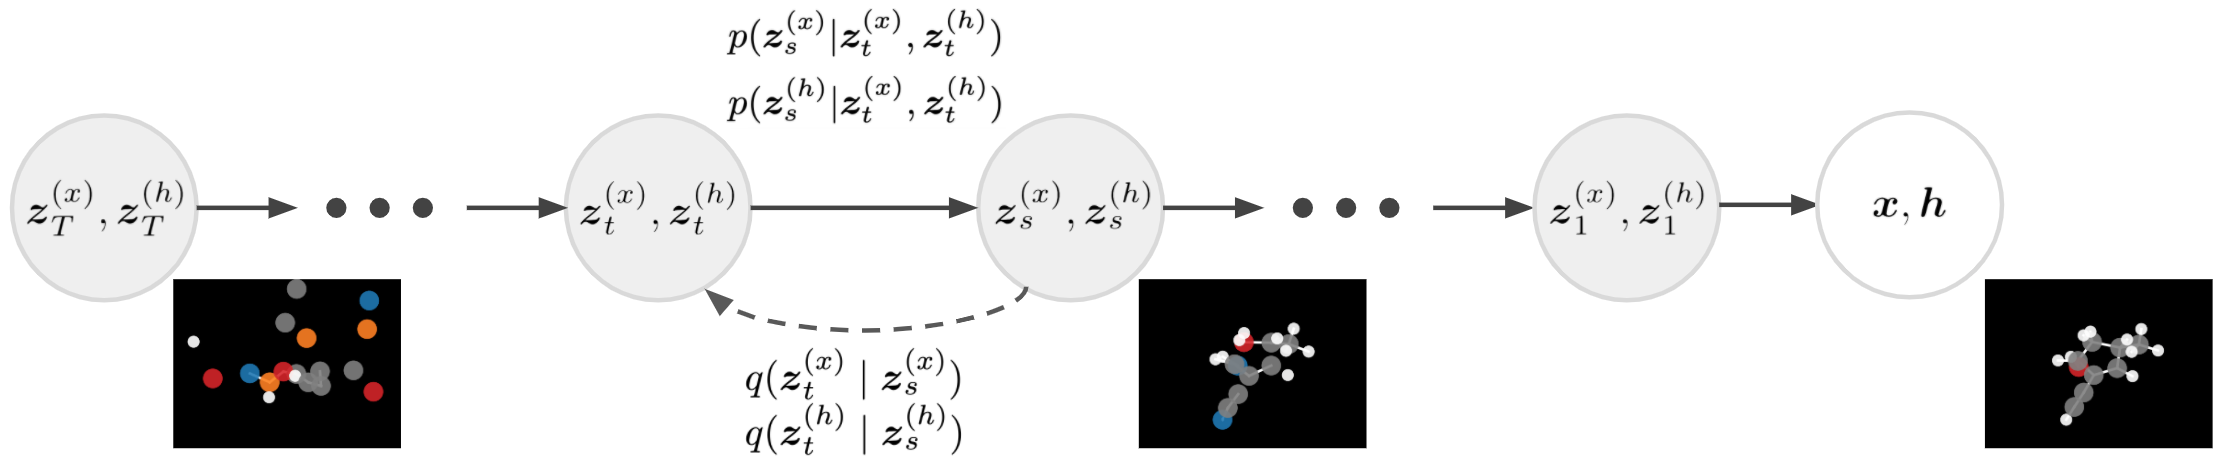
\includegraphics[width=0.42\textwidth]{figures/diffusion.png}
    \caption{The diffusion process of the molecule $\left[ \mathbf{x}, \mathbf{h} \right]$ in the latent space $\left[ \mathbf{z}^{(x)}, \mathbf{z}^{(h)} \right]$.}
    \label{fig:diffusion}
\end{figure}

\subsection{Graph Neural Networks}
Graph Neural Networks (GNNs) are a class of neural networks that operate on graph-structured data.
They are designed to capture the structure of the graph and the interactions between its nodes.
More precisely, \textit{a GNN is an optimizable transformation on all attributes of the graph (nodes, edges, and global attributes) 
that preserves graph symmetries}. (permutation invariance) \cite{gentle-intro-GNN}

\begin{figure}
    \centering
    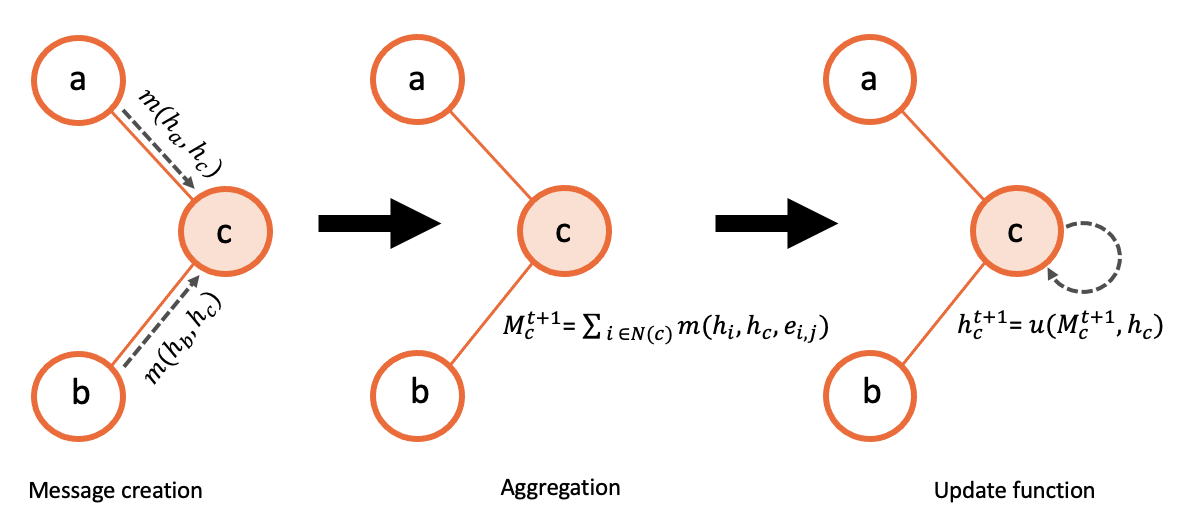
\includegraphics[width=0.42\textwidth]{figures/message_passing.png}
    \caption{The message passing scheme of a GNN.}
    \label{fig:message-passing}
\end{figure}

\subsection{Equivariance, Invariance, and the E(3) group}
Equivariance is a form of symmetry for functions. Roughly speaking, a function is equivariant to a group of transformations $G$ 
if and only if $\forall T\in G, f(T(x)) = T(f(x))$.
Likewise, invariance is when the function is constant under the action of the group i.e. $\forall T\in G, f(T(x)) = f(x)$.
In the context of molecule generation, we are interested in the spatial symmetries of the molecules. Indeed, only the relative positions of the atoms matter, not their absolute positions.
Therefore, we would want our generative model's final output to be invariant to the Euclidean group $E(3)$, which is the group of translations, rotations and reflections in 3D space.
Likewise, since we use diffusion to gradually denoise the molecule, we would want the denoising process to be equivariant to $E(3)$.
This inductive bias is expected to help the model learn the spatial structure of the molecules more efficiently i.e. the model will be able to generalize better and with less training data.

\subsection{E(3) Equivariant GNN}
In their paper, \cite{edm} propose a GNN architecture that is equivariant to the Euclidean group $E(3)$. To do so, they first define an Equivariant 
Graph Convolutional Layer (EGCL) that is equivariant to the Euclidean group $E(3)$. This layer is then stacked to form the Equivariant Graph Neural Network (EGNN).

The EGCL computes $\mathbf{x}^{t+1}, \mathbf{h}^{t+1} = \text{EGCL}(\mathbf{x}^t, \mathbf{h}^t)$ as follows:
\begin{gather}
    \mathbf{m}_{ij} = \phi_e(\mathbf(h)_i^t, \mathbf{h}_j^t, d_{ij}^2), \quad \tilde{e}_{ij} = \phi_{inf}(\mathbf{m}_{ij}) \\
    \mathbf{h}_i^{t+1} = \phi_h(\mathbf{h}_i^t, \sum_{j\neq i} \tilde{e}_{ij} \mathbf{m}_{ij}) \\
    x_i^{t+1} = x_i^t + \sum_{j\neq i} \frac{x_i^t - x_j^t}{d_{ij}+1} \phi_x(\mathbf{h}_i^t, \mathbf{h}_j^t, d_{ij}^2, a_{ij})
\end{gather}
where $\phi_e, \phi_{inf}, \phi_h, \phi_x$ are neural networks and $d_{ij}$ is the Euclidean distance between atoms $i$ and $j$.
Note that $\tilde{e}_{ij}$ implements an attention mechanism for the aggregation of the messages $\mathbf{m}_{ij}$.
Importantly, the EGCL is equivariant to actions the Euclidean group $E(3)$ on the atom positions $\mathbf{x}$ since replacing $\mathbf{x}_i^t$ by $R\mathbf{x}_i^t + t$ for any $R\in SO(3)$ and $t\in \mathbb{R}^3$ results in the same transformation on $\mathbf{x}_i^{t+1}$.
Besides, on can easily show by induction that the EGNN is also equivariant to $E(3)$ since it is a stack of EGCLs.

\subsection{Wrapping it together}
Finally, the Equivariant Diffusion Model (EDM) is obtained by combining the diffusion model and the EGNN.
The training objective is $\mathbb{E}_{t, \epsilon_t}[||\epsilon_t - \hat{\epsilon}_t||^2]$ where $\hat{\epsilon}_t$ i.e. we want to predict the noise.
We use the EGNN to predict the noise increment $\hat{\epsilon}_t$ given the noisy molecule $\left[ \mathbf{x}_t, \mathbf{h}_t \right]$ nad the time step $t$.
To be precise, we set $\hat{\epsilon}_t = \left[ \hat{\epsilon}_t^{(x)}, \hat{\epsilon}_t^{(h)} \right] 
= \text{EGNN}(\mathbf{z}_t^{(x)}, \mathbf{z}_t^{(h)}) - \left[ \mathbf{z}_t^{(x)}, \mathbf{0} \right]$. This recentering trick is necessary for translational equivariance of the EGNN. More details can be found in the original paper \cite{edm}.
Once the EGNN is trained, we can sample from the target distribution by starting from the simple distribution $\mathbf{z}_T \sim \mathcal{N}(0, I)$ and iteratively denoising it $T$ times to get $\mathbf{z}_0$.
We must then decode $\mathbf{z}_0 = \left[ \mathbf{z}_0^{(x)}, \mathbf{z}_0^{(h)} \right]$ to get the molecule $\left[ \mathbf{x}_0, \mathbf{h}_0 \right]$. Doing so is non-trivial since we have continuous (positions), categorical (atom type) and ordinal (charge) variables.
In the paper, the authors use Bayes rule and some approximations to decode $\mathbf{z}_0$.
\begin{itemize}
    \item The atom positions $\mathbf{x}_0$ are obtained by sampling from a gaussian distribution centered around $\mathbf{z}_0^{(x)}$ (plus a correction term)
    \item The atom type is obtained by sampling from a categorical distribution which essentially amounts to taking the nearest one-hot encoded vector to $(\mathbf{z}_0^{(h)})_{1:5}$
    \item The charge is obtained by sampling from a gaussian distribution centered around $(\mathbf{z}_0^{(h)})_6$ which essentially amounts to taking the nearest integer to $(\mathbf{z}_0^{(h)})_6$
\end{itemize}
In addition, the authors use a heuristic distance-based method to create the edges of the molecule. That is, for each pair of atoms $i$ and $j$, they compute the distance $d_{ij}$ 
and based on that distance and a table of bond lengths for these atoms they decide whether there is a bond between $i$ and $j$ and if so what type of bond it is.

Finally, note that since the initial distribution $\mathbf{z}_T \sim \mathcal{N}(0, I)$ is E(3)-invariant
\footnote{Note that no nonzero distribution can be translation invariant, since it wouldn't integrate to one. 
However, one can use distributions on the linear subspace of $(\mathbb{R}^3)^M$ such that the sum $\sum_i \mathbf{x}_i = \mathbf{0}$ i.e. the center of mass of the molecule is at the origin.
Xu et al \cite{xu} showed that such a linear subspace can be used consistently for diffusion.}
and the EGNN is E(3)-equivariant, the final distribution of the model is also E(3)-invariant. (this can be shown easily by induction)

\section{Limitations and Extensions}
\subsection{Evaluation Metrics}
Evaluation metrics for generation tasks are usually complex, and no consensus exists on the most appropriate criteria for different contexts. Here, we analyze the metrics used in this paper and highlight their limitations.

\subsubsection{Novelty}
Novelty, defined as the percentage of generated molecules which are both valid and not present in the training dataset, is one of the metrics employed. However, this metric can be misleading for \textit{exhaustive} datasets like QM9, which contains all "small" molecules satisfying certain constraints. For QM9, an ideal model should have near zero novelty, essentially reproducing the dataset molecules. Thus, novelty fails to capture the true quality of molecule generation \cite{vignac2022topnequivariantsetgraph} for QM9. If used as a sanity check to ensure the model is not generating entirely invalid molecules (a role that is not explicitly clarified in the paper), it can still provide some insight. However, it is insufficient as a standalone measure of model performance.

\subsubsection{Negative Log Likelihood}
Negative Log Likelihood (NLL), while central to the model’s training and optimization process, is not necessarily ideal for evaluating generation quality. NLL measures the closeness of the generated distribution to the dataset distribution but does not account for physical properties or structural validity. A model could achieve a low NLL while generating chemically invalid molecules. Additionally, the low NLL achieved by the EDM method compared to prior models could indicate sharper peaks (on the dataset $\mathcal{D})$ in the distribution, as suggested by the authors. While this reflects the model's ability to fit the data, it could also suggest overfitting, reducing generalization capability—a concern that warrants further exploration. Finally, we are dealing with multi-modal data (positions in 3D space and atom features) and thus a high NLL could be due to a given part of the input (e.g. the $z$ coordinate) fitted very well although another part of the input (e.g. the atom type) isn't fitted well.

\subsubsection{Stability}
The authors also evaluate stability metrics, such as atom stability (98.7\% on QM9) and molecule stability (82.0\% on QM9). The gap between these metrics highlights that while atomic-level features are well-represented, the model struggles to maintain coherent interatomic relationships and bond configurations. This discrepancy is significant but remains unexplored in the paper. Addressing the causes of this gap could provide insights into the limitations of the generative approach.

\subsubsection{QM9 vs. GEOM}
The authors emphasize strong performance on QM9, but the dataset's constrained diversity may lead to overfitting. In contrast, the GEOM dataset (which includes larger and more complex molecules) actually tests the model’s generalization ability. While EDM demonstrates close histogram distributions for derived energy metrics in GEOM, the stability of the generated molecules is not reported by the author but only added in the Appendix because it is abysmally low (2.8\%). The use of indirect metrics, like the Wasserstein distance of energy histograms, complicates the evaluation and adds little value in our view. While it shows that EDM aligns with the dataset’s energy distribution, there is no clear connection between this metric and the validity or stability of generated molecules, making the results harder to interpret.

\subsection{Potential Extensions}
\subsubsection{E(3) vs. SE(3) Equivariance}
The paper demonstrates that E(3) equivariance improves scalability and preserves some molecular symmetries. However, in general molecules are not stable under the action of E(3). Indeed, translation and rotation in space do not change the nature of a molecule but a reflexion can produce an enantiomere that has fundamentally different biological properties. Therefore SE(3) equivariance could be more appropriate for certain (chiral) molecules as it captures \textit{molecular orientation} whereas E(3) equivariance merely captures distances. While the paper does not explore this distinction, extending the framework to SE(3) equivariance could enhance the model’s capability to handle chiral molecules and other properties sensitive to spatial transformations. In other words, it seems to us that in the context of 3D molecule generation, SE(3) equivariance constitutes a better \textit{inductive bias} than E(3) equivariance.

\subsubsection{Incorporating Edge Features}
The current method for assessing bond validity relies on heuristics based on bond distances and valencies, tuned empirically for QM9. While effective for small molecules, this approach struggles with larger, more diverse datasets like GEOM-Drugs, where bond distances and aromaticity vary significantly. A more principled approach would incorporate bond types directly into the diffusion process using edge features, such as bond orders. Graph models leveraging edge features, like \cite{gilmer2017neuralmessagepassingquantum}, have shown that including this information improves molecular representations and downstream predictions. Integrating such features into diffusion models could enhance their alignment with chemical principles and improve stability metrics across datasets. We try incorporating edge information in Section 4 and show that it does in fact improve the performance of a graph neural network for classification.

\subsubsection{Incorporating Atom Counts}
Another limitation is the reliance on separate sampling of the number of atoms, \(M\), before molecule generation. Integrating \(M\) directly into the model as part of the generative process could improve flexibility and coherence. One could imagine another model whereby the number of atoms $M$ of the generated molecule is itself a latent variable which is part of the diffusion process. For instance, we could learn high-dimensional molecular embeddings and the corresponding decoder ; to generate samples, we would first perform diffusion in the embedding space and then decode the embedding into an actual molecule. However, building such a decoder seems non-trivial.

\subsection{Limited Applicability to Drug Discovery}
While the proposed method shows promise in generating small molecules, its applicability to drug discovery remains limited. Performance on structurally diverse or larger molecules is not adequately assessed. For example, in GEOM, the atom stability (85\%) remains relatively high, but the molecule stability (2.8\%) is very low, undermining its practical utility. Additionally, the model’s relevance to functional or biological properties, such as binding affinity or activity, is not evaluated. Incorporating these aspects would provide a more comprehensive understanding of its applicability to drug discovery and other real-world tasks.


\section{Experiments on toy model}
The key contribution of Hoogeboom's paper is the introduction of E(3)-equivariance. Their choice is motivated by the spatial symmetries of molecules. We aim to demonstrate the benefits of incorporating E(3)-equivariance in Graph Neural Networks (GNN) through a toy model experiment. We will focus on a regression task, which is less computationally intensive and sufficient to highlight the advantages of equivariant models over regular ones. Indeed, reproducing the paper's experiments is not feasible for students, as training takes about 7 days on GPUs. We will first present the dataset and task, then the models considered and implementation details. We will finally present the results of our experiments.

\subsection{Dataset}
The paper considers two molecule datasets: QM9 and GEOM. We will stick with QM9 for simplcity: it only contains small molecules with atoms in H, C, O, N, F. This allows us to focus on the model's ability to capture the spatial structure of the molecules without being overwhelmed by the complexity of larger molecules.
Additionnally, since QM9 has over 100,000 molecules, we filter to keep only molecules with 12 atoms or less. This brings us down to 4005 molecules.
Each sample in the dataset is a graph with several properties:
\begin{itemize}
    \item number of atoms $M$
    \item atom positions $\mathbf{x} \in (\mathbb{R}^3)^M$
    \item atom features $\mathbf{h} \in (\mathbb{R}^\text{nf})^M$ where $\text{nf} = 11$
    \begin{itemize}
        \item 1-5: atom type (one-hot: H, C, O, N, F)
        \item 6: atomic number (number of protons)
        \item 7: aromaticity (binary)
        \item 8-10: electron orbital hybridization (one-hot: sp, sp2, sp3)
        \item 11: number of hydrogens
    \end{itemize}
    \item graph edges (bonds) $\mathcal{E} \in \mathbb{R}^{2\times\text{\#edges}}$
    \item edge features $\mathcal{E}_\text{type} \in \mathbb{R}^{\text{\#edges}\times 4}$ (one-hot: single, double, triple, aromatic)
\end{itemize}
The QM9 dataset has 19 regression targets which are various physical properties of the molecules.
We will focus on the first target which is the dipole moment of the molecule. We chose this target because it is typically geometric so we expect to clearly see the benefits of 
incorporating E(3)-equivariance in the model.
We adopt a random split of 80\% training, 10\% validation, and 10\% test.
Finally, we normalize our regression target to have zero mean and unit variance.

\subsection{Layers}
All GNNs considered follow the same architecture:
\begin{enumerate}
    \item Linear layer to embed the atom features (which include the atom positions for MPNN): $(M,\text{nf}) \rightarrow (M, d_\text{embed})$
    \item Stacked GCL or EGCL layers (depending on the model) with $L$ layers: $(M, d_\text{embed}) \rightarrow (M, d_\text{embed})$ for GLC and $(M, d_\text{embed}+3) \rightarrow (M, d_\text{embed}+3)$ for EGCL
    \item Global mean pooling to aggregate the node features: $(M, d_\text{embed}) \rightarrow (d_\text{embed})$
    \item Linear layer to predict the regression target $(d_\text{embed},) \rightarrow (1,)$
\end{enumerate}

Let us describe the two types of layers considered.

The GCL layer computes $\mathbf{h}^{t+1} = \text{GCL}(\mathbf{h}^t)$ as follows:
\begin{enumerate}
    \item message $\mathbf{m}_{ij} = \phi_\mathbf{h}(\mathbf{h}_i, \mathbf{h}_j, \mathcal{E}_{ij})$
    \item aggregation $\mathbf{m}_i = \sum_{j\in\mathcal{N}(i)} \mathbf{m}_{ij}$ where $\mathcal{N}(i)$ is the set of neighbors of node $i$
    \item update $\mathbf{h}_i^{t+1} = \phi_\text{update}(\mathbf{h}^t, \mathbf{m}_i)$
\end{enumerate}

The EGCL layer computes $\mathbf{h}^{t+1}, \mathbf{x}^{t+1} = \text{EGCL}(\mathbf{h}^t, \mathbf{x}^t)$ as follows:
\begin{enumerate}
    \item message
    \begin{align*}
      \mathbf{m}_{ij}^\mathbf{h} &= \phi_\mathbf{h}(\mathbf{h}_i, \mathbf{h}_j, d_{ij}^2) \\
      \mathbf{m}_{ij}^\mathbf{x}& = \frac{\mathbf{x}_i - \mathbf{x}_j}{d_{ij}+1} \phi_\mathbf{x}(\mathbf{h}_i, \mathbf{h}_j, d_{ij}^2)
    \end{align*}
    \item aggregation
    \begin{align*}
      \mathbf{m}_i^\mathbf{h} &= \sum_{j\in\mathcal{N}(i)} \phi_\text{attention}(\mathbf{m}_{ij}) \mathbf{m}_{ij}^\mathbf{h} \\
      \mathbf{m}_i^\mathbf{x} &= \sum_{j\in\mathcal{N}(i)} \mathbf{m}_{ij}^\mathbf{x}
    \end{align*}
    \item update
    \begin{align*}
      \mathbf{h}_i^{t+1} &= \phi_\text{update}(\mathbf{h}_i^t, \mathbf{m}_i^\mathbf{h}) \\
      \mathbf{x}_i^{t+1} &= \mathbf{x}_i^t + \mathbf{m}_i^\mathbf{x}
    \end{align*}
\end{enumerate}

All the functions $\phi_\bullet$ are fully connected neural networks following the same architecture as in the original paper.
Both layers are trivially permutation equivariant i.e. if one permutes the node of the graph, the output of the layer will be permuted in the same way.
Besides, one can easily show from the equations that the EGCL is E(3)-equivariant i.e. $\mathbf{h}^t, R\mathbf{x}^t + \mathbf{t} = \text{EGCL}(\mathbf{h}^t, R\mathbf{x}^t + \mathbf{t})$ for all orthogonal matrix $R\in O(3)$ and translation vector $\mathbf{t} \in \mathbb{R}^3$.

Since our GNNs have stacked permutation equivariant layers and then a permutation invariant global mean pooling, they are permutation invariant.
Likewise, since $\mathbf{h}$ is E(3) invariant through the layers (as it only depends on the atom coordinates through the pairwise distances $d_{ij}$) and the output depends on $\mathbf{h}$ only (and not $\mathbf{x}$) after the layers, the GNNs are E(3) invariant.

\subsection{Models}

Taking inspiration from \cite{gnn-101}, we consider the following models:
\begin{itemize}
    \item MPNN: a Message Passing Neural Network (MPNN) built with stacked Graph Convolutional Layers (GCL)
    \item EGNN: an E(3)-equivariant GNN built with stacked E(3)-Equivariant Graph Convolutional Layers (EGCL)
    \item EGNN\_edge: same architecture as EGNN but using the edge features $\mathcal{E}_\text{type}$ as well when computing the messages
\end{itemize}
All models have $L=4$ layers and $d_\text{embed}=11$ (i.e. the same as the input dimension).
We also consider LinReg, a linear regression model (projects each atom to a scalar and sums them up to get the final prediction), for baseline comparison with the geometric models.
We expect poor performance as it doesn't leverage the graph structure of the molecules.

\begin{table}[h!]
\centering
\resizebox{0.5\textwidth}{!}{ % Resize the table to fit the text width
\begin{tabular}{|l|l|l|l|l|} \hline
\textbf{Model} & \textbf{Perm-Eq Layers} & \textbf{Perm-Inv} & \textbf{E(3)-Eq Layer} & \textbf{E(3)-Inv} \\ \hline
MPNN            & Yes                     & No                 & No                     & Yes                \\ \hline
EGNN            & Yes                     & Yes                & Yes                     & Yes                \\ \hline
EGNN\_edge      & Yes                     & Yes                & Yes                     & Yes                \\ \hline
LinReg          & No                     & Yes                 & No                     & Yes                \\ \hline
\end{tabular}
}
\caption{Symmetry Properties of the Different Models}
\end{table}

\subsection{Implementation details}
\begin{itemize}
    \item We use PyTorch Geometric to handle the graph data, with PyTorch as backend
    \item We use the Adam optimizer with a learning rate of $10^{-3}$ and a batch size of 64
    \item We use the ReduceLROnPlateau scheduler with a patience of 10 epochs, a factor of 0.9, and a minimum learning rate of $10^{-5}$
    \item We train each model for 500 epochs
    \item We use the mean squared error as the loss function
    \item We keep track of the learning rate, training loss and validation loss using WandB
    \item We train locally on CPU for simplicity. Each run is about 20 minutes on i7 with 8 cores.
\end{itemize}

\begin{figure}
    \centering
    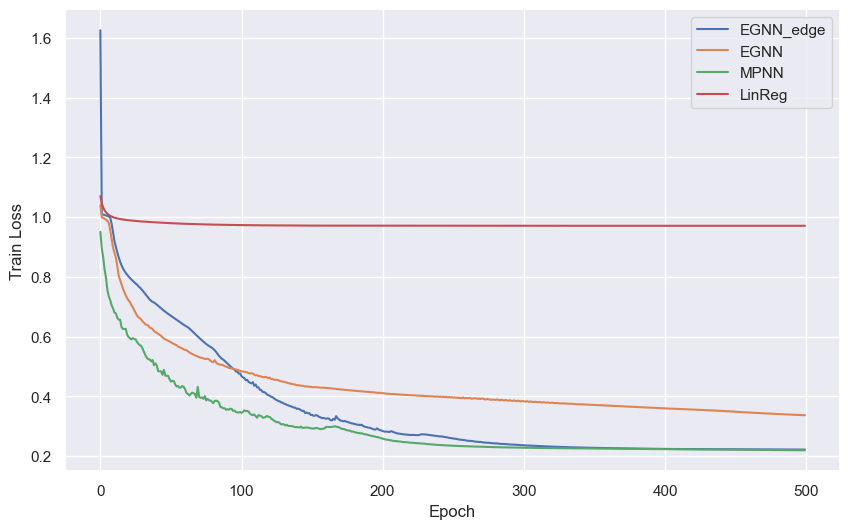
\includegraphics[width=0.42\textwidth]{figures/train_loss.png}
    \caption{Training loss. The LinReg model cannot even overfit the training data, illustrating the superiority of a graph-based approach.}
    \label{fig:training-loss}
\end{figure}

\begin{figure}
    \centering
    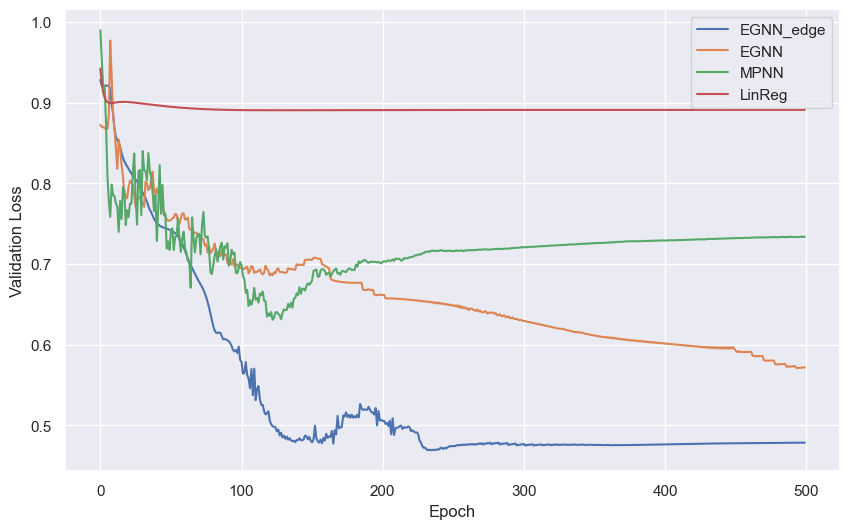
\includegraphics[width=0.42\textwidth]{figures/validation_loss.png}
    \caption{Validation loss. As expected, the EGNN models significantly outperform the MPNN model. In addition, the EGNN model lags behind the EGNN\_edge model, suggesting that incorporating edge features is beneficial.}
    \label{fig:validation-loss}
\end{figure}

\begin{figure}
    \centering
    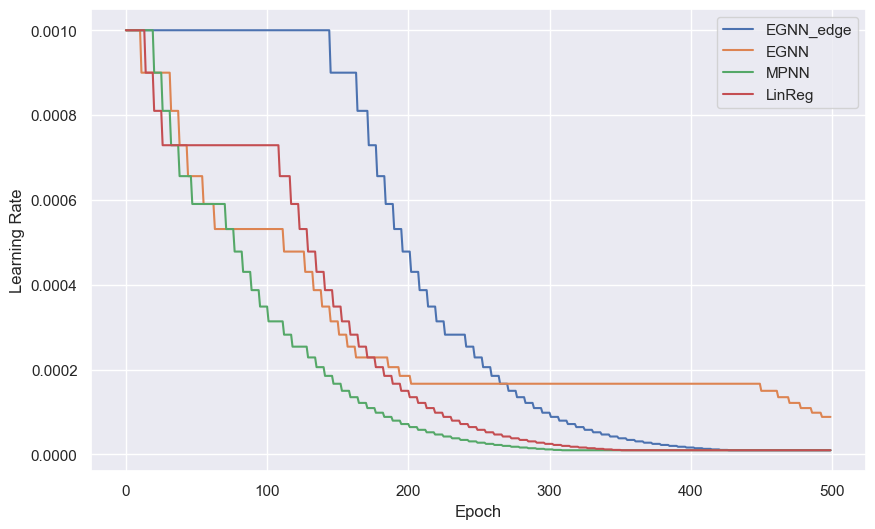
\includegraphics[width=0.42\textwidth]{figures/learning_rate.png}
    \caption{Learning Rate. All models have converged to a local minimum after 500 epochs, except the EGNN which is almost there.}
    \label{fig:learning-rate}
\end{figure}

\subsection{Comments}
The results are reported on three figures: the training loss, the validation loss, and the learning rate.

To begin with, the LinReg model performs very poorly as expected. Unlike its geometric counterparts, it cannot leverage the graph structure of the molecules and thus fails to learn anything meaningful.

Then, MPNN and EGNN\_edge have similar training losses but EGNN\_edge drastically outperforms MPNN on the validation set. This gap shows that EGNN\_edge's \textit{inductive bias} helps it \textit{generalize} better than MPNN.

Finally, EGNN is also significantly better than MPNN but learn much slower than EGNN\_edge. This suggests that incorporating edge features is beneficial to the model's performance.
Nonetheless, edge features can intuitively be inferred from the atom positions and types (using a distance-based heuristic like in the original paper), so the improvement is not as significant as the one brought by E(3)-equivariance.
That would explain why the EGNN is still learning and could potentially be as good as EGNN\_edge with more training. To verify this hypothesis, we trained the model for 1000 epochs, but the validation loss and training loss actually plateau around 500 epochs. There could be two reasons for that: either EGNN doesn't have enough capacity to infer the edge types itself (need for more layers or higher embedding dimension) or EGNN got stuck in a local minimum during training.

Finally, given the (intuitively) low complexity of our regression task, we expect that scaling up and fine-tuning the EGNN would lead to much better performance i.e. a much lower validation loss. However the goal of our toy experiment was solely to demonstrate the superiority of E(3) equivariant models over architectures which do not leverage the geometry of the problem. We leave the task of maximizing performance to researchers with professional computational resources.


\bibliographystyle{ACM-Reference-Format}
\bibliography{biblio}

\end{document}
